\section{QR code}
Quick Response (QR) codes are a type of matrix barcode designed for efficient data encoding and rapid scanning. They originated from the automotive industry but have since become widely used across various applications due to their versatility and capacity to store significant amounts of information.

\subsection{QR Structure}
A QR code is a two-dimensional matrix barcode designed to efficiently store and be readable from any angle. The code consists of black modules (squares) arranged on a white background in a grid pattern, allowing for rapid and error-resistant scanning. All QR Codes have a standard structure composed of the following elements:

\begin{figure}[h] % [h] forces the figure to be placed exactly here in the text
	\centering
	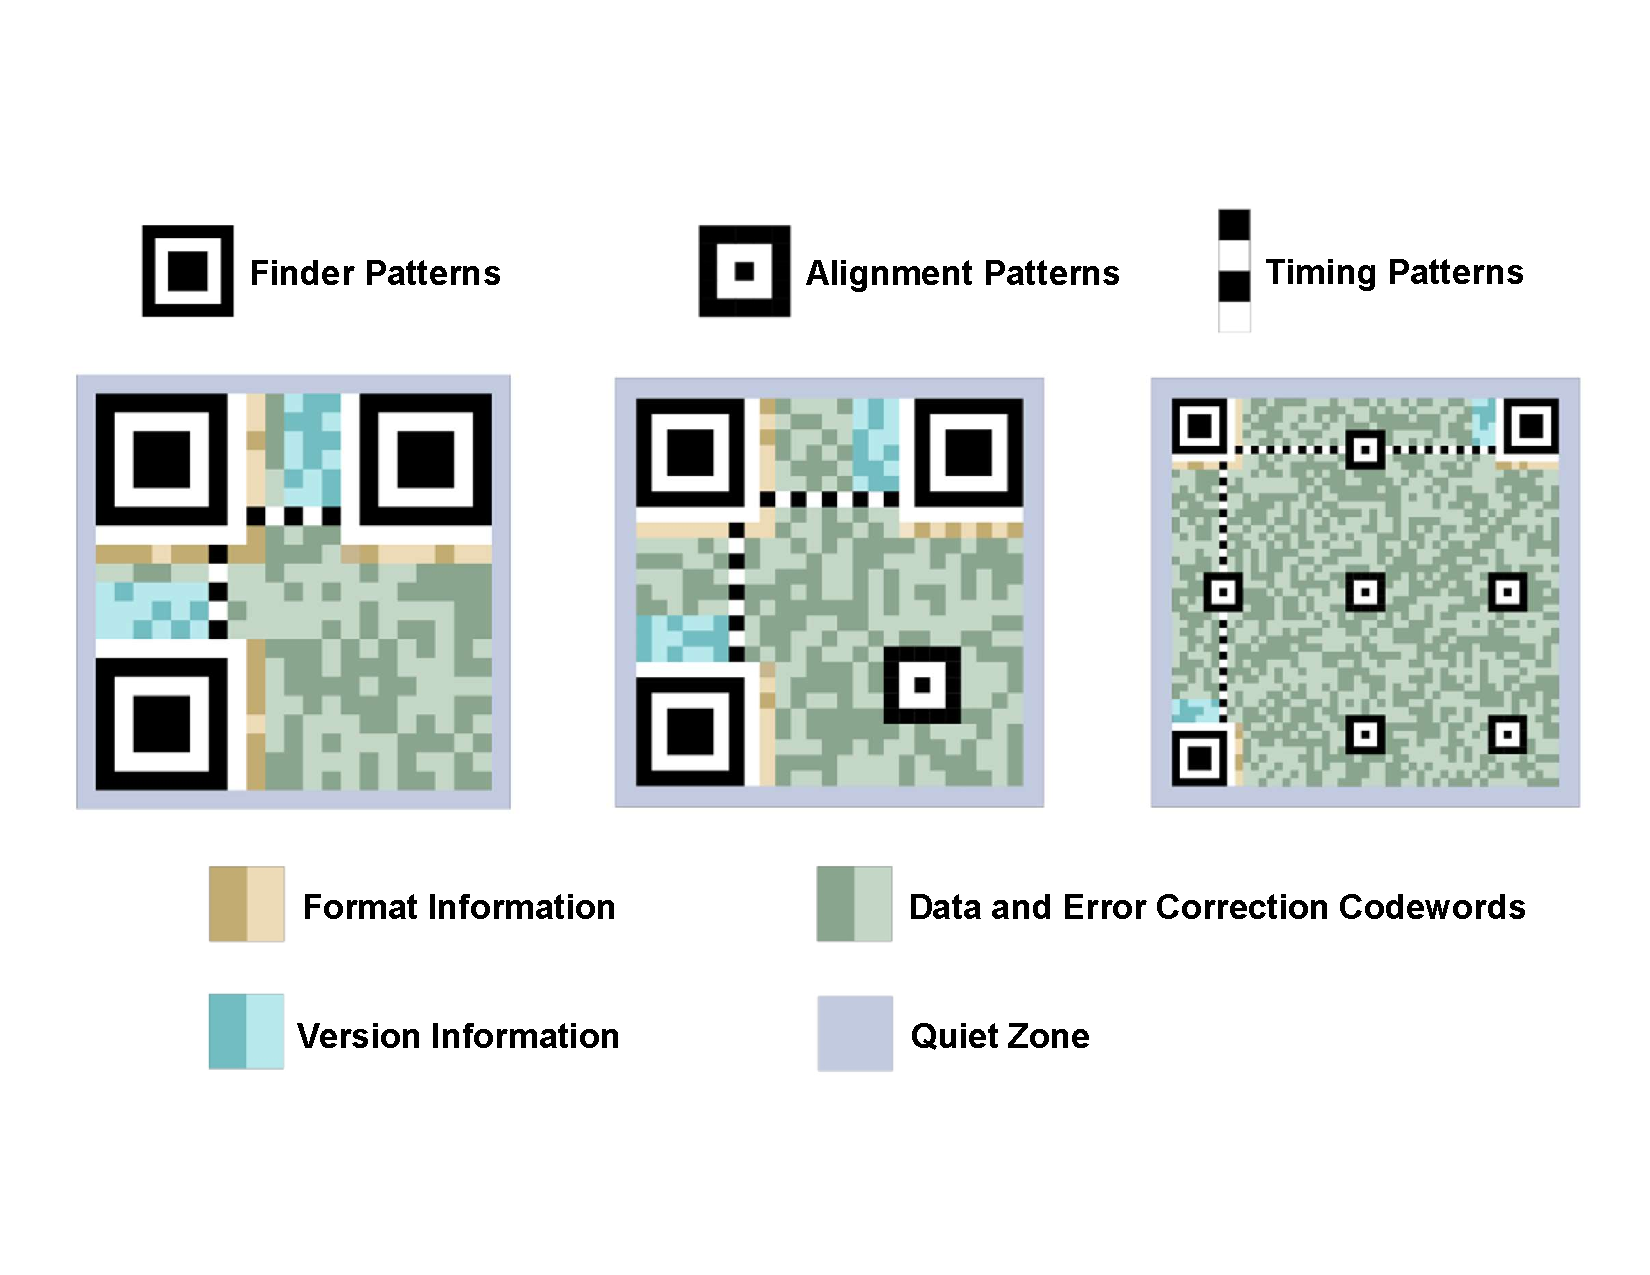
\includegraphics[width=15cm]{assets/ch2/qr_code_structure}
	\caption{QR code structure}
	\label{QR_code_structure}
\end{figure}

\subsubsection*{Finder Pattern}
The Finder Pattern is made up of three identical large square shapes positioned in the QR code. These patterns assist the scanning device in rapidly locating and orienting the QR code, regardless of its rotation or angle \cite{Tiwari2016}.

\subsubsection*{Alignment Pattern}
The Alignment Pattern is a smaller square that helps correct distortion and skewing of the QR code when viewed from different angles. It is especially crucial for larger QR codes that may be prone to bending or misalignment. The number of Alignment Patterns increases with the QR code version, such as in \ref{QR_code_structure}, which allows for better positional accuracy in larger codes \cite{Tiwari2016}.

\subsubsection*{Timing Pattern}
The Timing Pattern is made up of alternating black and white modules that are arranged in a straight line between the Finder Patterns. Timing Pattern is essential for defining the grid's structure and assists the scanner in establishing the size and coordinate system of the code \cite{Tiwari2016}.

\subsubsection*{Quiet Zone}
The Quiet Zone is the clear space around the entire QR code that separates the code from any surrounding graphics or text. This zone is crucial for the scanner to accurately identify the code's boundaries, ensuring reliable detection and reading \cite{Tiwari2016}.

\subsubsection*{Data and Error Correction}
The Data in a QR code contain encoded information such as text, URLs, or other data types. Error Corrections are created using error correction algorithms and are mixed with the data. These enable the QR code to recover and reconstruct the stored data, even if up to 30\% of the code is damaged or obscured \cite{Tiwari2016}.

\subsubsection*{Format and Version Information}
The Format Information provides details about the error correction level and data mask pattern used. This allows the decoder to interpret the QR code accurately \cite{Tiwari2016}.

\subsection{QR Code Versions and Types}
QR codes come in 40 versions, each representing a different size and data capacity. Version 1 contains 21 × 21 modules, while Version 40 has 177 × 177 modules. As the version number increases, so does the data capacity and the complexity of the code, making it capable of storing more information or supporting higher levels of error correction \cite{Tiwari2016}. 

\begin{figure}[h]
	\centering
	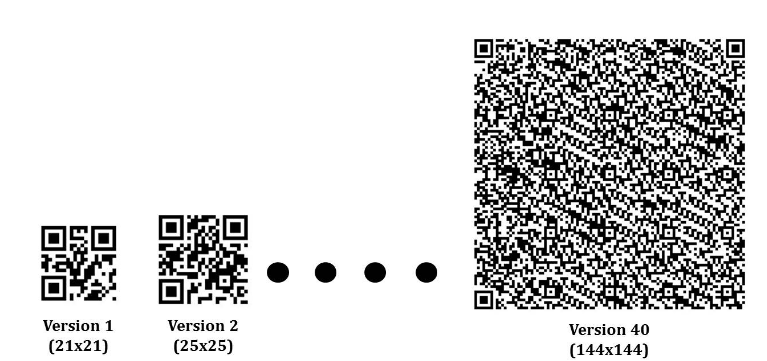
\includegraphics[width=10cm]{assets/ch2/qr_versions}
	\caption{QR codes Versions (adapted from \cite{Tiwari2016}).}
	\label{QR_versions}
\end{figure}


There are also specialized QR code types designed for specific applications:

\begin{itemize}
	\item \textbf{Micro QR Code}: Designed to be smaller and simpler, it uses only one Finder Pattern, making it more compact than traditional QR codes. It is often used when space is limited \cite{Tiwari2016}.
	\item \textbf{Logo QR Code}: Allows logos or images to be embedded within the QR code, enhancing the code's visual appeal for marketing or branding purposes \cite{Tiwari2016}.
	\item \textbf{iQR Code}: A flexible matrix-type QR code capable of being printed in various sizes and configurations, from small, high-capacity codes to large codes. It can store more data than standard QR codes and can be inverted or turned into dot patterns for direct part marking \cite{Tiwari2016}.
	\item \textbf{Encrypted QR Code}: Uses encryption techniques to secure the information encoded within, making it suitable for applications requiring data confidentiality \cite{Tiwari2016}.
\end{itemize}

\begin{figure}
	\centering
	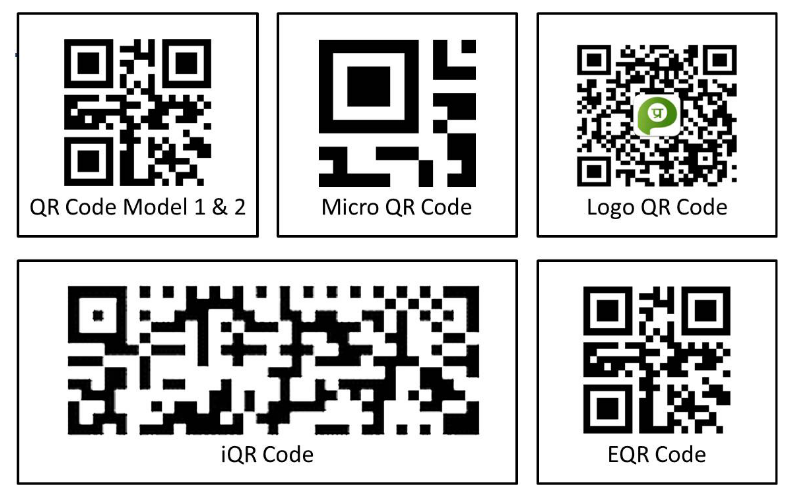
\includegraphics[width=0.7\linewidth]{assets/ch2/qr_codes_type}
	\caption{QR code types (adapted from \cite{Tiwari2016}).}
	\label{qr_code_type}
\end{figure}

\subsection{QR Code Encoding}  
The encoding process for a QR code involves converting data into a matrix of black and white modules. First, the input data is analyzed to determine the appropriate encoding mode, such as numeric, alphanumeric, byte, or Kanji. The data is then transformed into binary code, and error correction is added using Reed-Solomon algorithms, ensuring that the code can still be scanned if partially damaged \cite{Tiwari2016}.

Popular online tools for generating QR codes include:
\begin{itemize}
	\item \textbf{Online Tools}: These free online tools offer simple and fast solutions for both generating and decoding QR codes. QRickit allows users to decode QR codes from uploaded images, while GOQR.me provides various output formats, such as PNG, SVG, and EPS, making it versatile for different use cases \cite{QRCodeMonkey2024}\cite{QRTiger2024}.
	
	
\end{itemize}

For generating QR codes programmatically, popular libraries include:
\begin{itemize}
	\item \textbf{Python - PyQRCode}: A Python library that simplifies QR code creation, allowing output in SVG, PNG, and other formats \cite{PyQRCode2024}.
	\item \textbf{Java - ZXing (Zebra Crossing)}: An open-source library widely used for encoding QR codes in Java and Android applications \cite{ZXing2024}.
	\item \textbf{iOS - Core Image}: iOS provides native QR code generation capabilities via the `CIQRCodeGenerator` filter in the Core Image framework \cite{CoreImage2024}.
\end{itemize}

\subsection{QR Code Decoding}  
Decoding a QR code starts by scanning the Finder Patterns, which allow the scanner to properly align the code. Next, the Format Information is read to apply the correct error correction and mask pattern. Once decoded, the binary data is translated back into the original format (e.g., text, URL) \cite{Tiwari2016}.

Common online tools for decoding QR codes include:
\begin{itemize}
	\item \textbf{Online Tools}: These tools offer versatile QR code decoding solutions across platforms. ZXing is an open-source decoder integrated into Android and web applications, QRickit provides online QR code decoding from uploaded images, and Google Lens allows users to scan and decode QR codes directly via smartphone cameras \cite{ZXing2024, QRickit2024}.
	
\end{itemize}

For decoding programmatically, useful libraries include:
\begin{itemize}
	\item \textbf{Python - Segno}: A versatile Python library for generating and reading both QR and Micro QR codes \cite{Segno2024}.
	\item \textbf{Java - ZXing}: Provides decoding functionality along with encoding, and is widely used for mobile and web apps \cite{ZXing2024}.
	\item \textbf{iOS - AVFoundation}: iOS provides native support for scanning QR codes using the `AVCaptureMetadataOutput` class in the AVFoundation framework \cite{AVFoundation2024}.
\end{itemize}


